\documentclass[11pt, a4paper]{report}
\usepackage{graphicx}
\usepackage[table,xcdraw]{xcolor}
\usepackage{geometry}
\usepackage{float}
\usepackage{authblk}
\usepackage{anyfontsize}
\usepackage[document]{ragged2e}
\usepackage{titlesec}
\usepackage[parfill]{parskip}
\usepackage{color}   %May be necessary if you want to color links
\usepackage{hyperref}
\usepackage{caption}
\usepackage{tabularx}
\usepackage{longtable}
\usepackage{blindtext}
\hypersetup{
    colorlinks=true, %set true if you want colored links
    linktoc=all,     %set to all if you want both sections and subsections linked
    linkcolor=black,  %choose some color if you want links to stand out
}
\titleformat{\chapter}[hang] 
{\normalfont\huge\bfseries}{\chaptertitlename\ \thechapter:}{1em}{} 
\geometry{left=2.5cm,right=2.5cm,top=2.5cm,bottom=2.5cm}
\graphicspath{ {./images/} }

\begin{document}  
    \pagestyle{empty}
\centering
\fontsize{2cm}{2cm}\selectfont{System Requirements Document} \\
\vspace{2mm}
\fontsize{1cm}{1cm}\selectfont Audio digital signal processor \\
\vspace{2mm}
\large BeCreative Minor\\
\normalsize
\vspace{4cm}
\includegraphics[width=\linewidth]{3DR_P1_Perspective.png}\\
\vfill
\normalsize Busse Lommers \\
Robin van den Dungen \\
Mahmud Gürler \\
Silas Kamphuis \\
Hein Verhallen \\
Youri Tils \\
Ahmed Abdelrahim \\
Fontys Hogescholen, De Rondom 1, 5612 AP Eindhoven \\
\today

\begin{justify}


\newpage
\tableofcontents
\thispagestyle{empty}

\newpage
\pagestyle{plain}
\setcounter{page}{1}

\chapter*{Abbreviation List}

\begin{table}[!h]
	\centering
\begin{tabular}{|c|c|}
	\hline
\textbf{Abbreviation} & \textbf{Explanation}        	\\ \hline
DAC                   & Digital to analog converter 	\\ \hline
ADC                   & Analog to digital converter 	\\ \hline
RAM                   & Random acces memory 			\\ \hline
SINAD                 & Signal to noise and distortion 	\\ \hline
TRS                   & Tip ring sleeve connector(Jack)	\\ \hline
FPGA                  & Field programmable gate array 	\\ \hline
\end{tabular}
\caption{List of commonly used Abbreviations}
\label{Abbreviation list}
\end{table}

    \chapter{Introduction}
    The aim of this project was to fully develop an audio digital signal processor. During the project we researched and developed what it takes to make a working digital signal processor with a custom PCB and an FPGA-board. To house this we researched the ideal layout of the circuit boards and ports. 
\par
\noindent This paper shows the research and design process of the audio digital signal processor. It should contain the needed information to understand what was needed to visualize and create this product. 
Using our skills as engineering students we tried to develop an audio digital signal processor that has enhanced processing capabilities of audio, and is user-friendly and intuitive to use. 

    \chapter{Problem description}
    \section{Background}
%BACKGROUND

\noindent In the audio realm, digital signal processors (DSP) are employed to optimize sound systems. Since perfect speakers do not exist, all speakers inherently possess certain imperfections. However, a DSP can compensate for these imperfections and provide corrective measures. Additionally, DSPs are frequently utilized to enhance the dynamics of sound and imbue it with a distinct character or sensation.

\noindent As a group, we have chosen to develop an audio DSP for the BeCreative minor because we are eager to learn how audio DSPs function and how to create one ourselves. Our ultimate goal is to be able to utilize this audio DSP to enhance the listening experience of music by correcting for speaker imperfections and applying specific presets. The system must meet the requirements outlined in the System Requirements Document (SRD), but what is most important to us is the opportunity for learning and acquiring valuable knowledge throughout the process.


\section{Problem description}

\noindent When it comes to listening to music, it is crucial that the speakers are appropriately calibrated to both the surrounding environment and the position of the listener. This calibration is essential in order to achieve the best possible listening experience since sound pressure varies depending on the frequency at specific locations, characterized by nodes and antinodes. These nodes and antinodes shift throughout the space depending on the frequency. As a high fidelity (Hi-Fi) music listener, it is desirable to have the sound from all speakers reach you simultaneously. However, speakers are often not optimally positioned due to certain physical characteristics of the room. In cases where the speakers are not properly aligned with the surrounding environment, a digital signal processor can be utilized to rectify this issue. A DSP is a specialized processor designed specifically for digital signal processing.

\section{Project goals}

The goal of this project was to research how to make an audio-DSP. This raised the main research question: \textbf{“How to design an audio-DSP?”}. In the process of researching this an actual audio-DSP has been developed. From the main research question the following sub-research questions were derived:
\begin{itemize} %THIS IS TO MAKE LISTS
	\setlength\itemsep{-0.3em} %MAKES THE GAP SMALLER BETWEEN 2 ITEMS
	\item What is the best method for creating digital filters?
	\item What is the best method for creating digital effects?
	\item What is the most suitable anti-aliasing filter?
	\item What is the optimal needed roll-off for the anti-aliasing filter for a given bandwidth such that the noise can be negligible?
	\item What is the minimum sample frequency needed to capture the desired frequency spectrum?
	\item What is the minimum frequency range to be sampled to achieve sufficient detailed audio?
	\item What is the lowest allowable noise for decent audio?
	\item What analog to digital converter (ADC) resolution is needed such that the quantization error and noise level are on par?
	\item What ADC and digital to analog converter (DAC) architecture is most suitable for this application?
	\item What kind of processor is most suitable for this application?
	\item What is the permittable jitter for accurate audio?
	\item What is the maximum allowable ripple on the reference voltage for the ADC and DAC?
	\item How much RAM does the system need?
	\item How much flash does the system need?
	\item What power supply topology is best suited for each part of the system?
\end{itemize}



\par
\noindent
The audio system has some requirements to specify the final result. These requirements are derived with the “MoSCoW” method. It must be noted that the following requirements will be confirmed by the research that will be conducted.

	\newpage
	\section{Requirements}
	\begin{longtable}{|c|p{10cm}|c|c|}
		\hline
		\textbf{ID} & \textbf{Requirement} & \textbf{Priority} & \textbf{Status}\\ \hline 
		\textbf{U1} & \textbf{Inputs:} \newline
		•Two RCA audio inputs which work on a line level of 4dBu(±1,74V)\newline
		•Two 6,35mm TRS plug audio inputs which work on a line level of 4dBu(±1,74V)\newline
		•Two XLR audio inputs which work on a line level of 22dBu(±9,75)\newline
		•USB type B audio input & Must & Proposed\\ \hline

		\textbf{U2} & \textbf{Outputs:} \newline
		•Two RCA audio outputs which work on a line level of 4dBu(±1,74V)\newline
		•Two 6,35mm TRS plug audio outputs which work on a line level of 4dBu(±1,74V)\newline
		•Four XLR signal outputs which work on a line level of 22dBu(±9,75)
		 & Must & Proposed\\ \hline

		\textbf{U3} &The system should have a bandwidth (±3 dB) of at least 20 Hz up and till 20 kHz without any filters applied. 	& Must   & Proposed\\ \hline
		\textbf{U4} &The system has an Audio sample rate of at least 44.1 kHz 														& Must   & Proposed\\ \hline
		\textbf{U5} &The ADC and DAC resolution is at least 16-bit 																	& Must   & Proposed\\ \hline
		\textbf{U6} &The system has a propagation delay of less than 100ms without any filters applied 								& Must   & Proposed\\ \hline
		\textbf{U7} &User can select what input will be used via a user interface													& Must   & Proposed\\ \hline
		\textbf{U8} &User can select up to 4 effects to active on one channel at the same time 										& Must   & Proposed\\ \hline
		\textbf{U9} &User can configure each effect 																				& Must   & Proposed\\ \hline
		\textbf{U10} &The system must work stand alone and be configurable via a basic graphical user interface 					& Must   & Proposed\\ \hline
		\textbf{U11} &Effects are configurable per output channel, at least four different sound effects should be able to be applied to each signal output signal at the same time: \newline
		\begin{itemize}
			\setlength\itemsep{-0.4em}
			\item Distortion
			\item Reverb
			\item Gain
			\item Equalizer
			\item Delay
		\end{itemize}																												& Must 	 & Proposed\\ \hline
		\textbf{U12}  &The system should have a bandwidth (±1 dB) of at least 20 Hz up and till 20 kHz without any filters applied 	& Should & Proposed\\ \hline
		\textbf{U13}  &Audio sample rate of at least 96 kHz 																		& Should & Proposed\\ \hline
		\textbf{U14} & The ADC and DAC resolution is at least 24-bit. 																& Should & Proposed\\ \hline
		\textbf{U15} & Six XLR signal outputs work on a line level of 22 dBu (±9,75 V) 												& Should & Proposed\\ \hline
		\textbf{U16} & User can select up to 10 effects to be active in one channel at the same time. 								& Should & Proposed\\ \hline
		\textbf{U17} & Low enough jitter to not influence the audio quality too much 												& Should & Proposed\\ \hline
		\textbf{U18} & Local power supplies for different parts of the system 														& Should & Proposed\\ \hline
		\textbf{U19} & Low enough jitter to not influence the audio quality too much 												& Should & Proposed\\ \hline
		\textbf{U20} & Effects:\newline
		\begin{itemize}
			\setlength\itemsep{-0.3em}
			\item Phaser
			\item Tremelo
			\item Flanger
			\item Fuzz
			\item Overdrive
			\item Chorus
			\item Compressor
			\item Wah
			\item Looper
			\item Wow and flutter
			\item Modulator
			\item Echo
			\item Fade in
		\end{itemize}																												& Should & Proposed\\ \hline
		\textbf{U21} & Audio sample rate of at least 192 kHz 																		& Could  & Proposed\\ \hline
		\textbf{U22} & Touch screen user interface 																					& Could  & Proposed\\ \hline
		\textbf{U23} & Self-made mains power supply  																				& Won't  & Proposed\\ \hline
	\end{longtable}

\section{Project scope}

The project is conducted during the minor BeCreative at Fontys. This minor took 20 weeks and allowed the students to have a budget of €300,-. Thus after 20 weeks starting from 6-2-2023 an audio-DSP has been delivered within a budget of €300,-.
\par Weekly meetings were conducted with the project's assessor to keep the research and tasks on track.

\section{Boundary condition}

\section{Project approach}

The project is guided by a system of dividing tasks, having weekly meetings, and keeping each other up-to-date by asking questions outside of meetings. Research is devided and cohering tasks are assigned.

\section{Verification method}

At the end of the semester there should be a working audio DSP capable of the must-have requirements. 



    \chapter{Research}
    \section{Research objectives}

To come up with a working DSP system, research should be conducted to understand and implement certain subjects into the end-product. This research varies from firmware to hardware, but also more specific about electronical systems and digital filters.

\section{Research questions}

\begin{itemize} %THIS IS TO MAKE LISTS
	\setlength\itemsep{-0.3em} %MAKES THE GAP SMALLER BETWEEN 2 ITEMS
	\item What is the best method for creating digital filters?
	\item What is the best method for creating digital effects?
	\item What is the most suitable anti-aliasing filter?
	\item What is the optimal needed roll-off for the anti-aliasing filter for a given bandwidth such that the noise can be negligible?
	\item What is the minimum sample frequency needed to capture the desired frequency spectrum?
	\item What is the minimum frequency range to be sampled to achieve sufficient detailed audio?
	\item What is the lowest allowable noise for decent audio?
	\item What analog to digital converter (ADC) resolution is needed such that the quantization error and noise level are on par?
	\item What ADC and digital to analog converter (DAC) architecture is most suitable for this application?
	\item What kind of processor is most suitable for this application?
	\item What is the permittable jitter for accurate audio?
	\item What is the maximum allowable ripple on the reference voltage for the ADC and DAC?
	\item How much RAM does the system need?
	\item How much flash does the system need?
	\item What power supply topology is best suited for each part of the system?
\end{itemize}

\section{Research approach}

By looking at the research questions and project requirements, research can be done to finalize this project. Research consists of looking at other DSP systems, dissecting certain parts of the main PCB how it should work, and making calculations on certain electronical parts.  
\par
\noindent This type of research is considered qualitative research. Data collection and mathematical calculations can together prove or disprove certain ideas on the final product or on certain parts of the project.

\section{Results}
\begin{itemize} %THIS IS TO MAKE LISTS
	\setlength\itemsep{-0.3em} %MAKES THE GAP SMALLER BETWEEN 2 ITEMS
		\item The results of the research is listed below:
		\item The best method for creating digital filters is by utilizing the fast fourier transform (FFT).
		\item The sample frequency should be as high as possible in order to achieve the optimal roll-off for the anti-aliasing filter. 
		\item The minimum sample frequency should be 40Khz.
		\item The minimum frequency range for high quality audio is 20Hz to 20KHz.
		\item The lowest allowable noise is a SNR of 90dB and for HiFI audio it is a SNR of 120dB.
		\item The resolution needed for the ADC and DAC is 24 bit.
		\item The best ADC type is the TI PCM18xx Series.
		\item The best DAC type is the TI PCM17xx Series.
		\item The most suitable processor is a FPGA.
		\item The amount of flash needed depends highly on the program size.
		\item The best power supply topology's are: linear voltage regulator, buck converter and sepic converter.
		\item The USB implementation costs too much time for this project.
\end{itemize} 

    \chapter{Requirements}
    \section{Functional specifications}

The audio system has some requirements to specify the final result. These requirements are derived with the “MoSCoW” method. It must be noted that the following requirements will be confirmed by the research that will be conducted.

	\newpage
	\subsection{Requirements}
	\begin{longtable}{|c|p{10cm}|c|c|}
		\hline
		\textbf{ID} & \textbf{Requirement} & \textbf{Priority} & \textbf{Status}\\ \hline 
		\textbf{U1} & \textbf{Inputs:} \newline
		•Two RCA audio inputs which work on a line level of 4dBu(±1,74V)\newline
		•Two 6,35mm TRS plug audio inputs which work on a line level of 4dBu(±1,74V)\newline
		•Two XLR audio inputs which work on a line level of 22dBu(±9,75)\newline
		•USB type B audio input & Must & Proposed\\ \hline

		\textbf{U2} & \textbf{Outputs:} \newline
		•Two RCA audio outputs which work on a line level of 4dBu(±1,74V)\newline
		•Two 6,35mm TRS plug audio outputs which work on a line level of 4dBu(±1,74V)\newline
		•Four XLR signal outputs which work on a line level of 22dBu(±9,75)
		 & Must & Proposed\\ \hline

		\textbf{U3} &The system should have a bandwidth (±3 dB) of at least 20 Hz up and till 20 kHz without any filters applied. 	& Must   & Proposed\\ \hline
		\textbf{U4} &The system has an Audio sample rate of at least 44.1 kHz 														& Must   & Proposed\\ \hline
		\textbf{U5} &The ADC and DAC resolution is at least 16-bit 																	& Must   & Proposed\\ \hline
		\textbf{U6} &The system has a propagation delay of less than 100ms without any filters applied 								& Must   & Proposed\\ \hline
		\textbf{U7} &User can select what input will be used via a user interface													& Must   & Proposed\\ \hline
		\textbf{U8} &User can select up to 4 effects to active on one channel at the same time 										& Must   & Proposed\\ \hline
		\textbf{U9} &User can configure each effect 																				& Must   & Proposed\\ \hline
		\textbf{U10} &The system must work stand alone and be configurable via a basic graphical user interface 					& Must   & Proposed\\ \hline
		\textbf{U11} &Effects are configurable per output channel, at least four different sound effects should be able to be applied to each signal output signal at the same time: \newline
		\begin{itemize}
			\setlength\itemsep{-0.4em}
			\item Distortion
			\item Reverb
			\item Gain
			\item Equalizer
			\item Delay
		\end{itemize}																												& Must 	 & Proposed\\ \hline
		\textbf{U12}  &The system should have a bandwidth (±1 dB) of at least 20 Hz up and till 20 kHz without any filters applied 	& Should & Proposed\\ \hline
		\textbf{U13}  &Audio sample rate of at least 96 kHz 																		& Should & Proposed\\ \hline
		\textbf{U14} & The ADC and DAC resolution is at least 24-bit. 																& Should & Proposed\\ \hline
		\textbf{U15} & Six XLR signal outputs work on a line level of 22 dBu (±9,75 V) 												& Should & Proposed\\ \hline
		\textbf{U16} & User can select up to 10 effects to be active in one channel at the same time. 								& Should & Proposed\\ \hline
		\textbf{U17} & Low enough jitter to not influence the audio quality too much 												& Should & Proposed\\ \hline
		\textbf{U18} & Local power supplies for different parts of the system 														& Should & Proposed\\ \hline
		\textbf{U19} & Low enough jitter to not influence the audio quality too much 												& Should & Proposed\\ \hline
		\textbf{U20} & Effects:\newline
		\begin{itemize}
			\setlength\itemsep{-0.3em}
			\item Phaser
			\item Tremelo
			\item Flanger
			\item Fuzz
			\item Overdrive
			\item Chorus
			\item Compressor
			\item Wah
			\item Looper
			\item Wow and flutter
			\item Modulator
			\item Echo
			\item Fade in
		\end{itemize}																												& Should & Proposed\\ \hline
		\textbf{U21} & Audio sample rate of at least 192 kHz 																		& Could  & Proposed\\ \hline
		\textbf{U22} & Touch screen user interface 																					& Could  & Proposed\\ \hline
		\textbf{U23} & Self-made mains power supply  																				& Won't  & Proposed\\ \hline
	\end{longtable}

    
\section{Non-functional specifications}



    \chapter{Concept Development}
    \section{Concept overview}

\section{Architecture}

\section{Block diagrams}

\section{Modules}

\section{Design decisions}




    \chapter{Realization}
    \section{Hardware}

\section{Firmware}

\section{Software}

\section{User interface}



    \chapter{Verification}
    \section{Method}
Time has not yet allowed for the creation of a neat and detailed test plan. However, before the voltage regulator boards are soldered onto the main board, they need to be thoroughly tested to verify their functionality. The plan is to create a test table for this purpose, similar to the specification of ICs in datasheets.

\subsection{Hardware}
\subsubsection{Voltage regulators}
For the voltage regulator modules, the following parameters need to be measured to demonstrate proper operation:
-Thorough visual inspection, especially focusing on the soldering process. This includes checking for short circuits, open connections, solder balls, and other defects.
-The converter should be powered from a lab power supply with low current limit settings. In case of a short circuit or other module defect, the dissipated power will be limited, allowing for the identification and resolution of the issue.
-The output voltage of the converter should be observed using an oscilloscope. Attention should be paid to the absolute accuracy and the amplitude of the ripple voltage.
-The temperature of the PCB should be monitored to ensure that the module does not get too hot, which could potentially shorten its lifespan.

\subsubsection{Main board}
The functionality of the main board should be verified in the following manner:
-Perform a thorough visual inspection, with a focus on the soldering process. Check for short circuits, open connections, solder balls, and other defects.
-Power the main board from a lab power supply with low current limit settings. This will limit the dissipated power in case of a short circuit or module defect, enabling identification and resolution of the issue. A thermal camera can be used to inspect the PCB for hotspots.
-Verify the presence and correctness of all power rails.
-Verify that the output of the GPIO pins corresponds to the desired outcome.(e.g. check the SLCK).
-Next, apply a known signal (e.g., a 1kHz sinusoidal waveform with an amplitude of 100mV) to the various inputs of the audio-DSP. If no filters are selected and the audio-DSP is essentially in a pass-through state, the same signal should appear on the selected outputs. The accuracy of this signal can be verified using an audio analyzer such as the AP SYS 2700.

\subsection{Firmware}
The firmware can be tested by simulating the VHDL code in Modelsim. For this .do files are made to force input signals. Due to time constrains only the I2S decoder and encoder have been tested with real audio. 

\subsubsection{I2S decoder and encoder}
For testing the I2S decoder and encoder, they are wired in series. So when a random data pattern is going in the decoder the encoder should output the same data pattern.

\subsubsection{I2C master}
The I2C master is tested by simply writing and reading data with the protocol and verifying that the protocol works correctly according to the I2C protocol standards. 

\subsubsection{State-space BPF}
The state-space BPF is tested by inputting a sine wave outputted from a sine wave generator. By using a sine wave as an input it is very easy to expect the outcome. For instance when having the BPF resonance frequency at 1kHz and inputting a 1kHz sine wave, it is expected that the output sine wave has no attenuation compared to the input sine wave. And when the frequency of the input sine wave does not match that of the BPF resonance frequency, it will be attenuated. 

\section{Results}

\subsection{Hardware}

\subsubsection{Buck}
Due to the limited time, this verification has not been done yet.

\subsubsection{SEPIC}
The output voltage of the SEPIC with a 1A load is shown in figure \ref{fig:Verification_SEPIC_1A_Load}. It can be observed that the ripple voltage reasonably matches the calculated and simulated values. In figure \ref{fig:Verification_SEPIC_1A_Load}, some very high-frequency voltage spikes are visible on the output, but the author of this report is convinced that this is due to the large ground loop during measurement because no ground spring was available for the oscilloscope probe at Fontys. For this reason, the author quickly improvised a solution using a piece of wire, as shown in figure \ref{fig:Improvised_GND_spring}. This reduced the measured ripple voltage from over 40mVpp to approximately 4mVpp.

\subsubsection{Linear voltage regulator}
After conducting a thorough visual inspection, it became apparent that a thorough cleaning of the PCB was necessary. This was because the solder paste used left behind a significant amount of residue. Therefore, the linear voltage regulators were cleaned in an ultrasonic cleaner.

Subsequently, the linear regulators were connected to a lab power supply with current limiting. However, it quickly became evident that the regulators were not functioning properly. After performing several simulations in LTspice, it was suspected that the LEDs, which serve as low-noise voltage references, might have been soldered incorrectly. However, after consulting the datasheet again with several group members, it was confirmed that the LEDs were indeed soldered correctly according to the datasheet.

Since no other plausible causes emerged after further investigation, it was decided to desolder one of the LEDs and measure it out of circuit using a multimeter to determine its polarity and threshold voltage. To the astonishment of the group, it was discovered that the Broadcom datasheet for the HSMH-C170 LED did not match the LEDs actually supplied. The polarity marking in the datasheet was the exact opposite of the actual component. It is unknown whether an incorrect batch was delivered or if the datasheet itself is genuinely incorrect.
%https://nl.mouser.com/datasheet/2/678/AV02_0551EN_DS_HSMx_Cxxx_25Mar2022-1827675.pdf

\subsubsection{Main board}
\paragraph{inspection} Before connecting every module together and placing every component on the main board it is indeed ascertain that the board has flux and solder paste residue together with solder balls that can cause short circuits, therefore the PCB will be cleaned in the ultrasonic bath, before doing this it is important to know which components are suitable for this. The relays and electrolytic capacitors are not suitable for this, therefore they are soldered after cleaning.  visual inspection has been done on the main board and the power delivery modules. In the second visual inspection there are no signs of shorts and the components are connected properly.

\paragraph{Power inspection}

The PCB is inspected and no short circuit is detected. The next step is to check all the power modules within the PCBA with current limiting, so that the board will not be catch on fire if there is somehow still a short. This has been done with a power supply limited to 1A. All the power rails are tested and every power delivery module is working properly at the desired voltage. The 12V buck converter that is going to the FPGA is tested separately first with four 33 resistors connected in parallel which will give 1.5A of current at 12V. The buck was still below 50°C. 

\subsection{Firmware}
\subsubsection{I2S encoder and decoder}
The results of this test can be found in figure \ref{fig:i2s-dec-enc}. These results show that the I2S encoder and decoder work as expected. 

\begin{figure}[!ht]
    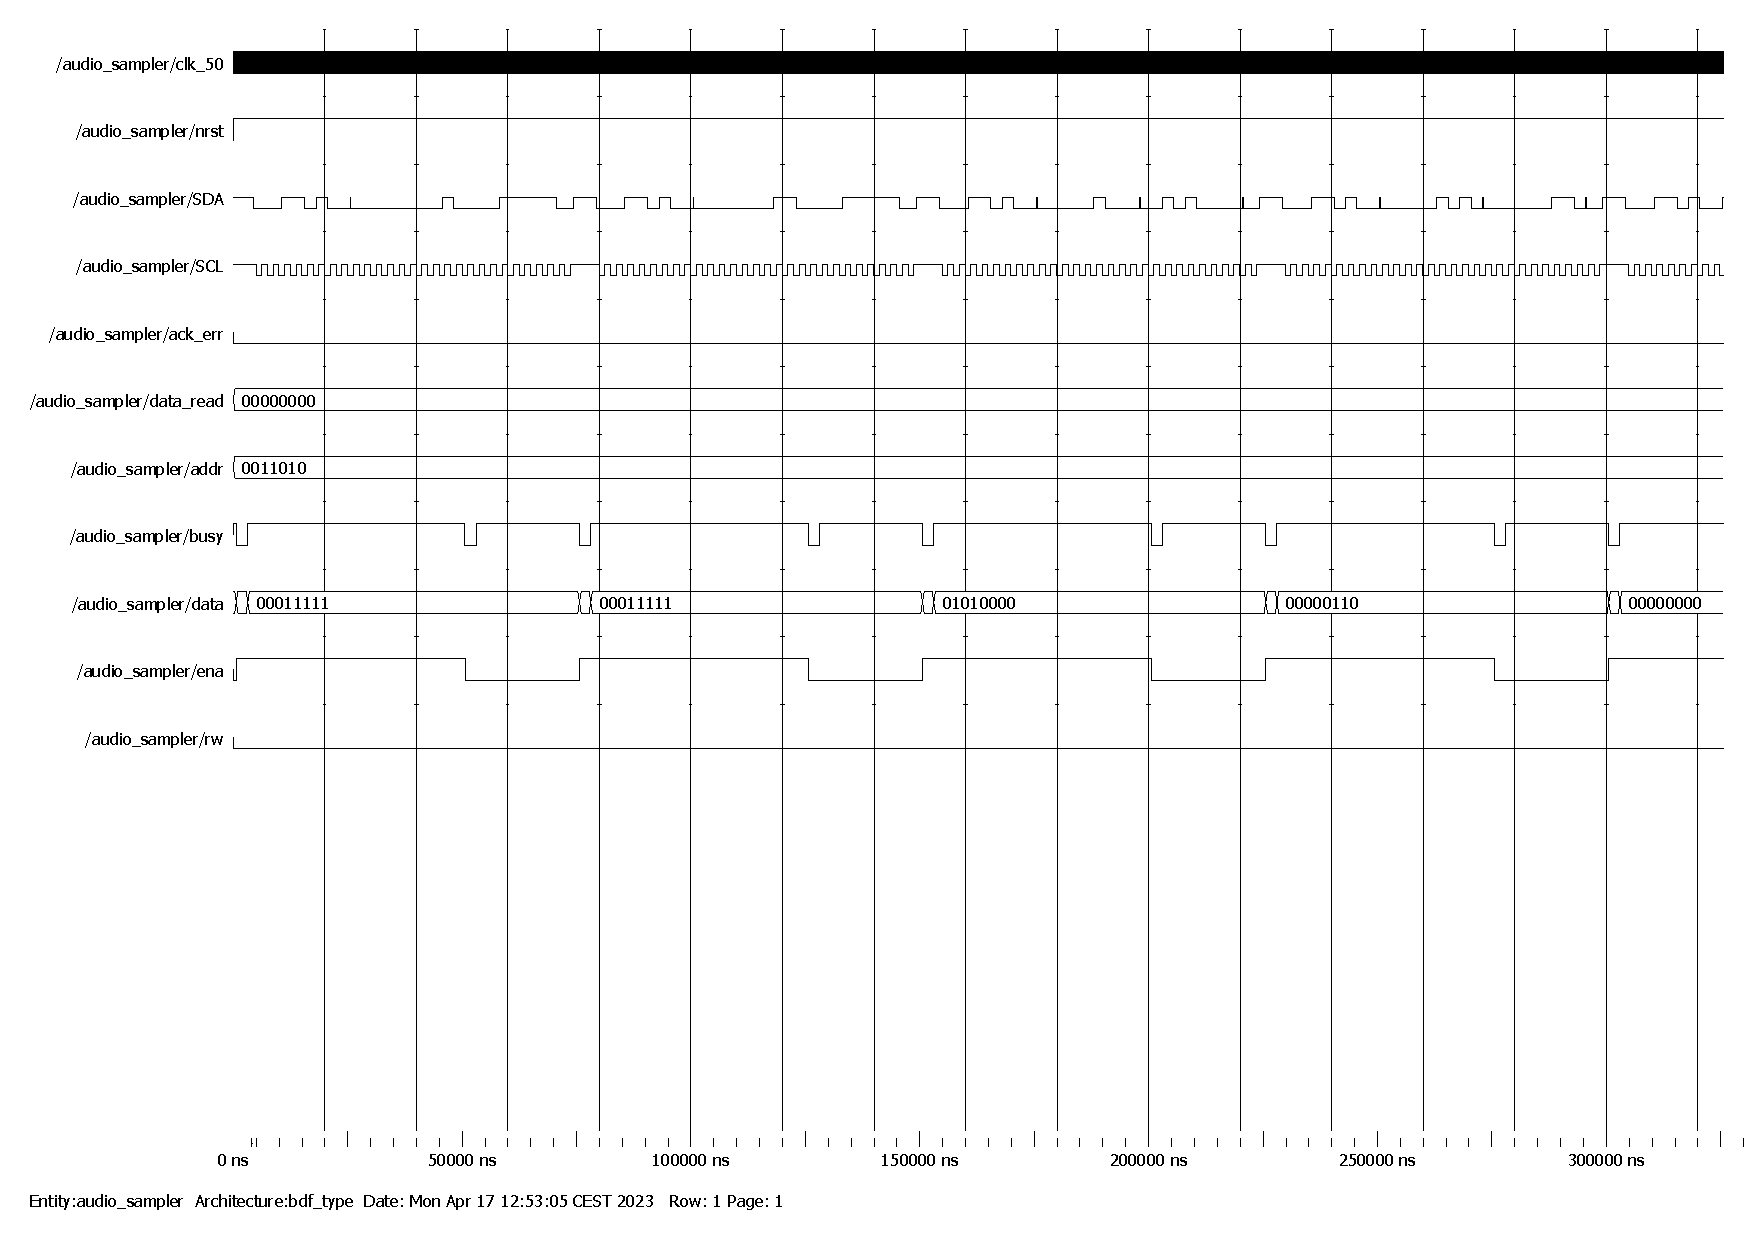
\includegraphics[width=\linewidth, keepaspectratio]{Audio_sampler_result.png}
    \caption{Simulation result of I2S decoder and encoder}
    \label{fig:i2s-dec-enc}
\end{figure}

\subsubsection{I2C master}
The results can be seen in figure \ref{fig:i2c-master}. In this result it can be seen that the I2C master works as expected according to the protocol standards.

\begin{figure}[!ht]
    \includegraphics[width=\linewidth, keepaspectratio]{I2C_master_result.png}
    \caption{Simulation result of I2C master}
    \label{fig:i2c-master}
\end{figure}

\subsubsection{State-space BPF}
Due to time constrains the BPF has not yet been tested in Modelsim. 

\section{Conclusions}

\subsection{Hardware}

\subsubsection{Buck}
Due to the limited time, this verification has not been done yet.

\subsubsection{SEPIC}
The SEPIC appears to be functioning well after some quick measurements. With an input voltage of +12V, it generates a stable -15V output voltage, and the voltage ripple remains nearly constant regardless of the output current. This aligns with the calculations and simulations. Additionally, the amplitude of the output ripple voltage closely matches the calculated and simulated values.

\subsubsection{Linear voltage regulator}
Due to the limited time, this verification has not yet been completed.

\subsubsection{Main board}
Due to the limited time, this verification has not been done yet.

\subsection{Firmware}
The I2S decoder, I2S encoder and I2C master work as expected. Therefore it is possible to sample audio using the ADC and DAC of the FPGA board. This has been tested and verified that this works. 

Due to time constrains further testing and implementation of the effects has not been conducted. 


    \chapter{Conclusions}
    We weten nog niet of het werkt?

    \chapter{Recommendations}
    Due to time constraints the project has not yet been finished. Most parts have been tested and work as expected, but some parts still have to be implemented and tested according to the planning. Some more time is needed to finish the Project.
\par
\noindent The following recommendations have been made to help the project work/ work better:

\begin{itemize}
    \setlength\itemsep{-0.3em} %MAKES THE GAP SMALLER BETWEEN 2 ITEMS
    \item Do not use FFT for the processing, use a direct approach instead or use a way more powerful processor
    \item Look into the clock signals from the FPGA board to the main PCB
    \item Investigate if there are other FPGA boards available which do support the needed 24.576 MHz output frequency on their GPIO pins
    \item Indicate on the UI screen which option is selected
    \item Make a less enthusiastic project planning
\end{itemize}

    \chapter*{References}
    \addcontentsline{toc}{chapter}{References}  

    \chapter*{Appendices}
    \addcontentsline{toc}{chapter}{Appendices}  
    
    \end{justify}
\end{document}